\documentclass[preprint,12pt]{elsarticle}

\usepackage{amssymb}
\usepackage{amsmath}

% EXTRAS FOR QUARTO

\usepackage{fancyvrb}
\usepackage{booktabs}
\usepackage{longtable}
\usepackage{multirow}
\usepackage{siunitx}

\usepackage{float}
\usepackage{xcolor}
\usepackage{framed}
\usepackage{calc}
\usepackage{longtable}
\usepackage{hyperref}

\providecommand{\tightlist}{%
  \setlength{\itemsep}{0pt}\setlength{\parskip}{0pt}}

\NewDocumentCommand\citeproctext{}{}
\NewDocumentCommand\citeproc{mm}{%
  \begingroup\def\citeproctext{#2}\cite{#1}\endgroup}
\makeatletter
 % allow citations to break across lines
 \let\@cite@ofmt\@firstofone
 % avoid brackets around text for \cite:
 \def\@biblabel#1{}
 \def\@cite#1#2{{#1\if@tempswa , #2\fi}}
\makeatother

\newlength{\cslhangindent}
\setlength{\cslhangindent}{1.5em}
\newlength{\csllabelwidth}
\setlength{\csllabelwidth}{3em}
\newenvironment{CSLReferences}[2] % #1 hanging-indent, #2 entry-spacing
 {\begin{list}{}{%
  \setlength{\itemindent}{0pt}
  \setlength{\leftmargin}{0pt}
  \setlength{\parsep}{0pt}
  % turn on hanging indent if param 1 is 1
  \ifodd #1
   \setlength{\leftmargin}{\cslhangindent}
   \setlength{\itemindent}{-1\cslhangindent}
  \fi
  % set entry spacing
  \setlength{\itemsep}{#2\baselineskip}}}
 {\end{list}}
\newcommand{\CSLBlock}[1]{\hfill\break#1\hfill\break}
\newcommand{\CSLLeftMargin}[1]{\parbox[t]{\csllabelwidth}{\strut#1\strut}}
\newcommand{\CSLRightInline}[1]{\parbox[t]{\linewidth - \csllabelwidth}{\strut#1\strut}}
\newcommand{\CSLIndent}[1]{\hspace{\cslhangindent}#1}

\newcommand{\VerbBar}{|}
\newcommand{\VERB}{\Verb[commandchars=\\\{\}]}
\DefineVerbatimEnvironment{Highlighting}{Verbatim}{commandchars=\\\{\}}
\definecolor{shadecolor}{RGB}{248,248,248}
\newenvironment{Shaded}{\begin{snugshade}}{\end{snugshade}}
\newcommand{\AlertTok}[1]{\textcolor[rgb]{0.94,0.16,0.16}{#1}}
\newcommand{\AnnotationTok}[1]{\textcolor[rgb]{0.56,0.35,0.01}{\textbf{\textit{#1}}}}
\newcommand{\AttributeTok}[1]{\textcolor[rgb]{0.77,0.63,0.00}{#1}}
\newcommand{\BaseNTok}[1]{\textcolor[rgb]{0.00,0.00,0.81}{#1}}
\newcommand{\BuiltInTok}[1]{#1}
\newcommand{\CharTok}[1]{\textcolor[rgb]{0.31,0.60,0.02}{#1}}
\newcommand{\CommentTok}[1]{\textcolor[rgb]{0.56,0.35,0.01}{\textit{#1}}}
\newcommand{\CommentVarTok}[1]{\textcolor[rgb]{0.56,0.35,0.01}{\textbf{\textit{#1}}}}
\newcommand{\ConstantTok}[1]{\textcolor[rgb]{0.00,0.00,0.00}{#1}}
\newcommand{\ControlFlowTok}[1]{\textcolor[rgb]{0.13,0.29,0.53}{\textbf{#1}}}
\newcommand{\DataTypeTok}[1]{\textcolor[rgb]{0.13,0.29,0.53}{#1}}
\newcommand{\DecValTok}[1]{\textcolor[rgb]{0.00,0.00,0.81}{#1}}
\newcommand{\DocumentationTok}[1]{\textcolor[rgb]{0.56,0.35,0.01}{\textbf{\textit{#1}}}}
\newcommand{\ErrorTok}[1]{\textcolor[rgb]{0.64,0.00,0.00}{\textbf{#1}}}
\newcommand{\ExtensionTok}[1]{#1}
\newcommand{\FloatTok}[1]{\textcolor[rgb]{0.00,0.00,0.81}{#1}}
\newcommand{\FunctionTok}[1]{\textcolor[rgb]{0.00,0.00,0.00}{#1}}
\newcommand{\ImportTok}[1]{#1}
\newcommand{\InformationTok}[1]{\textcolor[rgb]{0.56,0.35,0.01}{\textbf{\textit{#1}}}}
\newcommand{\KeywordTok}[1]{\textcolor[rgb]{0.13,0.29,0.53}{\textbf{#1}}}
\newcommand{\NormalTok}[1]{#1}
\newcommand{\OperatorTok}[1]{\textcolor[rgb]{0.81,0.36,0.00}{\textbf{#1}}}
\newcommand{\OtherTok}[1]{\textcolor[rgb]{0.56,0.35,0.01}{#1}}
\newcommand{\PreprocessorTok}[1]{\textcolor[rgb]{0.56,0.35,0.01}{\textit{#1}}}
\newcommand{\RegionMarkerTok}[1]{#1}
\newcommand{\SpecialCharTok}[1]{\textcolor[rgb]{0.00,0.00,0.00}{#1}}
\newcommand{\SpecialStringTok}[1]{\textcolor[rgb]{0.31,0.60,0.02}{#1}}
\newcommand{\StringTok}[1]{\textcolor[rgb]{0.31,0.60,0.02}{#1}}
\newcommand{\VariableTok}[1]{\textcolor[rgb]{0.00,0.00,0.00}{#1}}
\newcommand{\VerbatimStringTok}[1]{\textcolor[rgb]{0.31,0.60,0.02}{#1}}
\newcommand{\WarningTok}[1]{\textcolor[rgb]{0.56,0.35,0.01}{\textbf{\textit{#1}}}}

%%%%%%%%%%%%%%%%%%%

\journal{Computational Statistics \& Data Analysis}

\begin{document}

\begin{frontmatter}

\title{`cpp11armadillo': An `R' Package to Use the Armadillo C++
Library}

\author{Mauricio Vargas Sepúlveda and Jonathan Schneider Malamud}

\affiliation{organization={Department of Political Science, Munk School
of Global Affairs and Public Policy, and Department of Electrical and
Computer Engineering, University of Toronto},
            addressline={1 Devonshire Pl}, 
            city={Toronto},
            postcode={M5S 3K7}, 
            state={Ontario},
            country={Canada}}

\begin{abstract}
This article introduces `cpp11armadillo', an R package that integrates
the highly efficient Armadillo C++ linear algebra library with R through
the `cpp11' interface. Designed to offer significant performance
improvements for computationally intensive tasks, `cpp11armadillo'
simplifies the process of integrating C++ code into R. This package is
particularly suited for R users requiring efficient matrix operations,
especially in cases where vectorization is not possible. Our benchmark
demonstrate substantial speed gains over native R functions and
Rcpp-based setups.
\end{abstract}

\begin{keyword}
Numerical linear algebra \sep Programming languages \sep Object-oriented programming
\MSC[2024] 65F05 - 65F50 \sep 68N15 \sep 68N19
\end{keyword}

\end{frontmatter}

\section{Introduction}\label{introduction}

As R continues to grow in popularity for statistical computing and data
analysis, it can create bottlenecks when working with large datasets.
The need to interface with lower-level languages like C++ to bypass
these bottlenecks has led to the development of tools like `Rcpp'
(Eddelbuettel and Francois 2011), and more recently, `cpp11' (Vaughan,
Hester, and François 2023).

`cpp11armadillo' is a novel package that builds upon the existing
Armadillo C++ library (Sanderson and Curtin 2016) to provide high-level
access to efficient linear algebra operations directly from R. The
existing `RcppArmadillo' (Eddelbuettel and Sanderson 2014) already
offers this, and `cpp11armadillo' offers an alternative with modern C++
features, where we highlight vendoring, that can improve performance and
simplify the its usage.

\section{Features}\label{features}

`cpp11armadillo' simplifies C++ integration by leveraging the `cpp11'
package (Vaughan, Hester, and François 2023), which is designed to
reduce the complexity of including C++ code in R. Its core features
include:

\begin{itemize}
\item
  High-Performance Matrix Operations: By using Armadillo, cpp11armadillo
  allows users to perform matrix multiplications, inversions, and
  decompositions with minimal overhead. These operations are, for some
  cases, several times faster than their R counterparts.
\item
  Simplified Syntax: Armadillo offers a user-friendly syntax similar to
  that of `MATLAB' (Sanderson and Curtin 2016), making it accessible to
  R users without requiring an extensive background in C++.
\item
  Modern C++ Support: `cpp11armadillo' supports C++11 and newer
  standards, enabling efficient memory management, parallel
  computations, and advanced templates, all integrated into an R
  workflow.
\item
  Integration with R: The package allows direct manipulation of R data
  structures (e.g., vectors, matrices) in C++, providing a seamless
  workflow between the two languages without requiring manual data
  conversion (e.g., such as exporting data to CSV files and continously
  reading them in R to use the C++ output or vice versa).
\end{itemize}

\section{Background}\label{background}

The R programming language was not designed for high-performance
computing, it was created to offer ready-made statistical functions for
the end-user, and its interpreted nature can lead to slow execution
times for computationally intensive tasks (Wickham et al. 2019; `R` Core
Team 2024). The same applies to Python and other high-level languages.

Compiled languages like C++ offer significant performance improvements
due to their direct access to hardware resources and efficient memory
management. The counterpart is that C++ has a steep learning curve and
it is less user-friendly than R. C++ goals are different, it is designed
to be fast and efficient, and it is not focused on statistical computing
but on general-purpose programming (Stroustrup 2012).

However, bottlenecks in R can be solved by using vectorized operations
instead of writing loops, which treats data objects as a whole instead
of element-wise (Burns 2011). There are cases where vectorization is not
possible or challenging to implement (Burns 2011), and this is where
`cpp11armadillo' comes in and it offers data structures and functions
that are not available in R that facilitate the implementation of loops
and other operations (`R` Core Team 2024; Sanderson and Curtin 2016).

Even in spite of these difficulties to work with large datasets or
computationally intensive tasks, R is a growing popularity language for
statistical computing and data analysis, and its community has created
tools to integrate it with SQL databases for memory-efficient data
access (Wickham, Ooms, and Müller 2023). There are multiple ways to
measure a language popularity, and one of them is the number of R
questions in Stack Overflow, which has been increasing over the years as
shown in the following plot (Stack Overflow 2024).

\begin{figure}[H]

{\centering 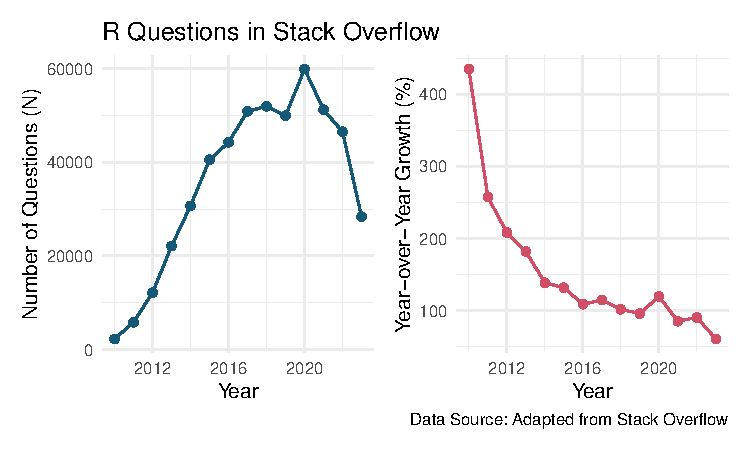
\includegraphics{cpp11armadillo_files/figure-pdf/stackoverflow-1.pdf}

}

\caption{R Questions in Stack Overflow increase from 2,260 in 2010 to
28,385 in 2023 with a peak of 59,895 in 2020.}

\end{figure}%

\section{Modern C++ features}\label{modern-c-features}

`cpp11' is a modern rewrite of the C++ interface for R, designed to
improve safety, performance, and ease of use. It enforces copy-on-write
semantics to prevent unintended modifications to data, ensuring that
changes to objects do not affect other references. Additionally, `cpp11'
provides safer access to R's C API, reducing runtime errors in C++ code.
It also supports ALTREP objects for efficient memory management and
deferred computations, making it ideal for handling large datasets. By
using UTF-8 strings throughout, `cpp11' ensures robust handling of
datasets created in different countries where encodings vary (Vaughan,
Hester, and François 2023).

Built on C++11 features like smart pointers and lambdas, `cpp11' offers
a more straightforward and efficient implementation compared to previous
bindings. Its header-only design eliminates ABI compatibility issues,
making it easier to integrate and manage in projects. `cpp11' also
compiles faster, uses less memory, and grows vectors more efficiently,
optimizing performance when dealing with large amounts of data. These
improvements make `cpp11' a powerful, streamlined tool for developers
who need reliable, high-performance C++ bindings for R (Vaughan, Hester,
and François 2023).

Following from `cpp11', `cpp11armadillo' leverages these modern C++
features to provide a seamless interface between R and the Armadillo
library, offering high-performance linear algebra operations with
minimal overhead. Besides the technical aspects, `cpp11armadillo' offers
vendoring, something not available in `RcppArmadillo', which can
simplify the installation process and reduce dependency issues,
especially when working in environments with restricted access to the
Internet. For instance, the
\href{https://docs.scinet.utoronto.ca/index.php/Niagara_Quickstart}{Niagara
Supercomputer} that we use at the University of Toronto has restricted
access to the Internet, and vendoring can simplify the installation
process.

Vendoring is a well-known concept in the Go community, and it consists
in copying the dependency code directly into a project's source tree.
This approach ensures that dependencies remain fixed and stable,
preventing any external changes from inadvertently breaking the project.
While vendoring offers stability, it comes with trade-offs. The primary
advantage is that updates to the `cpp11armadillo' library will not
disrupt existing code, and it also copies `cpp11' C++ headers. However,
the drawbacks include an increase in package size and the loss of
automatic updates, meaning that bug fixes and new features will only be
available when manually updated.

In other words, vendoring allows the package creator to provide a
dependency-free package that can be installed in any environment without
requiring the end user to install `cpp11' nor `cpp11armadillo'. This
approach makes `cpp11armadillo' a dependency for the developer but not
for the end user.

\section{Usage}\label{usage}

To use `cpp11armadillo', users must first install the package from CRAN
or GitHub. The package includes the Armadillo library, no additional
installation is required. The following code shows how to install the
package:

\begin{Shaded}
\begin{Highlighting}[]
\FunctionTok{install.packages}\NormalTok{(}\StringTok{"cpp11armadillo"}\NormalTok{)}

\CommentTok{\# or}
\NormalTok{remotes}\SpecialCharTok{::}\FunctionTok{install\_github}\NormalTok{(}\StringTok{"pachadotdev/cpp11armadillo"}\NormalTok{)}
\end{Highlighting}
\end{Shaded}

Once installed, users can use the provided package template function to
create a new package that uses C++ code with Armadillo. The package
template includes simple examples and all the necessary files to compile
the code and install the new R package. The following code shows how to
create a new package:

\begin{Shaded}
\begin{Highlighting}[]
\NormalTok{cpp11armadillo}\SpecialCharTok{::}\FunctionTok{create\_package}\NormalTok{(}\StringTok{"cpp11newpackage"}\NormalTok{)}
\end{Highlighting}
\end{Shaded}

The package
\href{https://pacha.dev/cpp11armadillo/index.html}{vignettes} cover the
directories organization and the necessary steps to build an R package
with relatively low setup efforts.

It is important to note that `cpp11armadillo' only work within an R
package, and it is not possible to compile individual C++ scripts on the
fly. This design choice ensures that the R and C++ code is organized
following the organization described in Wickham and Bryan (2023).

\section{Benchmarks}\label{benchmarks}

In order to evaluate the performance of `cpp11armadillo', we compared it
with native R functions and `RcppArmadillo'. We focused on a single test
consisting in computing the Balassa Index (Vargas Sepulveda 2020).

The R code for the Balassa Index computation is as follows:

\begin{Shaded}
\begin{Highlighting}[]
\NormalTok{balassa\_r }\OtherTok{\textless{}{-}} \ControlFlowTok{function}\NormalTok{(X) \{}
\NormalTok{  B }\OtherTok{\textless{}{-}} \FunctionTok{t}\NormalTok{(}\FunctionTok{t}\NormalTok{(X }\SpecialCharTok{/} \FunctionTok{rowSums}\NormalTok{(X)) }\SpecialCharTok{/}\NormalTok{ (}\FunctionTok{colSums}\NormalTok{(X) }\SpecialCharTok{/} \FunctionTok{sum}\NormalTok{(X)))}
\NormalTok{  B[B }\SpecialCharTok{\textless{}} \DecValTok{1}\NormalTok{] }\OtherTok{\textless{}{-}} \DecValTok{0}
\NormalTok{  B[B }\SpecialCharTok{\textgreater{}=} \DecValTok{1}\NormalTok{] }\OtherTok{\textless{}{-}} \DecValTok{1}
\NormalTok{  B}
\NormalTok{\}}
\end{Highlighting}
\end{Shaded}

The C++ code for the Balassa Index computation from an R matrix is as
follows:

\begin{Shaded}
\begin{Highlighting}[]
\NormalTok{Mat}\OperatorTok{\textless{}}\DataTypeTok{double}\OperatorTok{\textgreater{}}\NormalTok{ balassa\_armadillo}\OperatorTok{(}\AttributeTok{const}\NormalTok{ doubles\_matrix}\OperatorTok{\textless{}\textgreater{}\&}\NormalTok{ x}\OperatorTok{)} \OperatorTok{\{}
\NormalTok{  mat X }\OperatorTok{=}\NormalTok{ as\_Mat}\OperatorTok{(}\NormalTok{x}\OperatorTok{);}
\NormalTok{  mat B }\OperatorTok{=}\NormalTok{ X}\OperatorTok{.}\NormalTok{each\_col}\OperatorTok{()} \OperatorTok{/}\NormalTok{ sum}\OperatorTok{(}\NormalTok{X}\OperatorTok{,} \DecValTok{1}\OperatorTok{);}
\NormalTok{  B }\OperatorTok{=}\NormalTok{ B}\OperatorTok{.}\NormalTok{each\_row}\OperatorTok{()} \OperatorTok{/} \OperatorTok{(}\NormalTok{sum}\OperatorTok{(}\NormalTok{X}\OperatorTok{,} \DecValTok{0}\OperatorTok{)} \OperatorTok{/}\NormalTok{ accu}\OperatorTok{(}\NormalTok{X}\OperatorTok{));}
\NormalTok{  B}\OperatorTok{.}\NormalTok{elem}\OperatorTok{(}\NormalTok{find}\OperatorTok{(}\NormalTok{B }\OperatorTok{\textless{}} \DecValTok{1}\OperatorTok{)).}\NormalTok{zeros}\OperatorTok{();}
\NormalTok{  B}\OperatorTok{.}\NormalTok{elem}\OperatorTok{(}\NormalTok{find}\OperatorTok{(}\NormalTok{B }\OperatorTok{\textgreater{}=} \DecValTok{1}\OperatorTok{)).}\NormalTok{ones}\OperatorTok{();}
  \ControlFlowTok{return}\NormalTok{ B}\OperatorTok{;}
\OperatorTok{\}}
\end{Highlighting}
\end{Shaded}

After implementing the C++ computation in `cpp11armadillo' and
`RcppArmadillo', we compared the execution time of obtaining the Balassa
index year by year for the 2002-2020 period, which involves 19 matrices
with an approximate dimension of \(230 \times 5,100\). After a build
time of 4.4s for `cpp11armadillo' and 9.5s for `RcppArmadillo'. The
following plot reveals almost identical execution times for the
Armadillo function called from `cpp11armadillo' and `RcppArmadillo' with
a marginal advantage for `cpp11armadillo', and both are significantly
faster than the base R function.

\begin{figure}[H]

{\centering 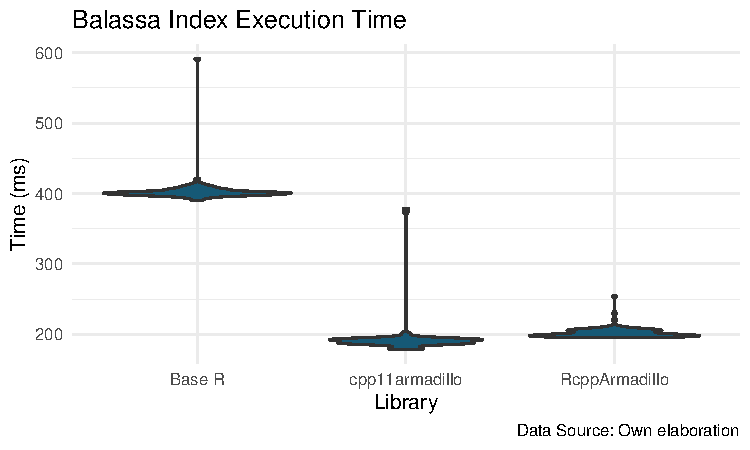
\includegraphics{cpp11armadillo_files/figure-pdf/benchmark-1.pdf}

}

\caption{Balassa Index execution time reveals speed gains of around 50\%
for Armadillo implementations compared to base R.}

\end{figure}%

\newpage

The benchmarks were conducted on a ThinkPad X1 Carbon Gen 9 with the
following specifications:

\begin{itemize}
\tightlist
\item
  Processor: Intel Core i7-1185G7 with eight cores
\item
  Memory: 16 GB LPDDR4Xx-4266
\item
  Operating System: Pop!\_OS 22.04 based on Ubuntu 22.04
\item
  R Version: 4.4.1
\item
  BLAS Library: OpenBLAS 0.3.20
\end{itemize}

\subsection{Conclusion}\label{conclusion}

`cpp11armadillo' provides a simple and efficient way to integrate C++
code with R, leveraging the `cpp11' package and the Armadillo library.
It simplifies the process of writing C++ code for R users, allowing them
to focus on the logic of the algorithm rather than the technical details
of the integration. It can help to solve performance bottlenecks in `R'
code by using the efficient linear algebra operations provided by
Armadillo in cases where vectorization is challenging. `RcppArmadillo'
is a popular package for this purpose, it has existed for nearly a
decade, `cpp11armadillo' offers a different approach with similar
performance.

\phantomsection\label{refs}
\begin{CSLReferences}{1}{0}
\bibitem[\citeproctext]{ref-burns2011}
Burns, Patrick. 2011. \emph{The r Inferno}. Lulu.

\bibitem[\citeproctext]{ref-eddelbuettel2011}
Eddelbuettel, Dirk, and Romain Francois. 2011. {``Rcpp: {Seamless} {R}
and {C}++ {Integration}.''} \emph{Journal of Statistical Software} 40
(April): 1--18. \url{https://doi.org/10.18637/jss.v040.i08}.

\bibitem[\citeproctext]{ref-eddelbuettel2014}
Eddelbuettel, Dirk, and Conrad Sanderson. 2014. {```Rcpparmadillo`:
{Accelerating} {R} with High-Performance {C}++ Linear Algebra.''}
\emph{Computational Statistics \& Data Analysis} 71 (March): 1054--63.
\url{https://doi.org/10.1016/j.csda.2013.02.005}.

\bibitem[\citeproctext]{ref-r2024}
`R` Core Team. 2024. \emph{`R`: A Language and Environment for
Statistical Computing}. Vienna, Austria: `R` Foundation for Statistical
Computing. \url{https://www.R-project.org/}.

\bibitem[\citeproctext]{ref-sanderson2016}
Sanderson, Conrad, and Ryan Curtin. 2016. {``Armadillo: A Template-Based
c++ Library for Linear Algebra.''} \emph{Journal of Open Source
Software} 1 (2): 26. \url{https://doi.org/10.21105/joss.00026}.

\bibitem[\citeproctext]{ref-stackoverflow2024}
Stack Overflow. 2024. {``{Stack} {Exchange} {Data} {Explorer}.''}
\url{https://data.stackexchange.com/stackoverflow/query/new}.

\bibitem[\citeproctext]{ref-stroustrup2012}
Stroustrup, Bjarne. 2012. {``Tour : {Standard} {C}++.''}
\url{https://isocpp.org/tour}.

\bibitem[\citeproctext]{ref-vargassepulveda2020}
Vargas Sepulveda, Mauricio. 2020. {``Economiccomplexity: {Computational}
{Methods} for {Economic} {Complexity}.''} \emph{Journal of Open Source
Software} 5 (46): 1866. \url{https://doi.org/10.21105/joss.01866}.

\bibitem[\citeproctext]{ref-cpp11}
Vaughan, Davis, Jim Hester, and Romain François. 2023. \emph{`Cpp11`: A
c++11 Interface for r's c Interface}.
\url{https://CRAN.R-project.org/package=cpp11}.

\bibitem[\citeproctext]{ref-wickham2019}
Wickham, Hadley, Mara Averick, Jennifer Bryan, Winston Chang, Lucy
D'Agostino McGowan, Romain François, Garrett Grolemund, et al. 2019.
{``Welcome to the Tidyverse.''} \emph{Journal of Open Source Software} 4
(43): 1686. \url{https://doi.org/10.21105/joss.01686}.

\bibitem[\citeproctext]{ref-wickham2023}
Wickham, Hadley, and Jennifer Bryan. 2023. \emph{R Packages}. "O'Reilly
Media, Inc.".

\bibitem[\citeproctext]{ref-rpostgres}
Wickham, Hadley, Jeroen Ooms, and Kirill Müller. 2023.
\emph{`Rpostgres`: C++ Interface to PostgreSQL}.
\url{https://CRAN.R-project.org/package=RPostgres}.

\end{CSLReferences}

\bibliographystyle{elsarticle-num-names} 
\bibliography{references.bib}

\end{document}
